\lab{Python}{Object Oriented Programming}{Graphical User Interfaces}
\objective{Illustrate the uses of OOP in programming graphical user interfaces}

Object oriented programming is used in a variety of situations.
Expressing some problems in an objected oriented context yield very nice, elegant solutions.
One problem that is very nicely expressed in the paradigm of object oriented programming is creating a graphical user interface.

In this lab, we will be using Python and Qt4 (with bindings provided by PySide or PyQt) to create a web navigator.
It will be able to load and render webpages and will have basic navigation functionality such as back, forward, stop, and reload.
This project is designed to be used for demonstration purposes only and no effort is made to make this program secure.
We need to import the libraries we will need for this project.
Qt, the framework we will leverage, is a cross-platform application framework.
It is very comprehensive and powerful and supports a number of platforms including Linux, OS X, Windows, etc.
At the time of writing, PyQt and PySide support Qt version 4.8.
\begin{lstlisting}
import sys
from PyQt4 import QtCore, QtGui
from PyQt4 import QtWebKit
\end{lstlisting}

\emph{Widgets} in Qt are objects that represent various elements of a GUI.
These widgets take care of drawing and refreshing the graphical display of the element as well as abstracting the behavior and defining ways to interact with the widget.
We are going to create our own widget, called \li{WebNavigator}, that will represent a simple web navigator.
We start by inheriting all the properties and methods of a generic widget.
\begin{lstlisting}
class WebNavigator(QtGui.QWidget):
    def __init__(self, home="about:blank"):
        super(WebNavigator, self).__init__()
        self.home = QtCore.QUrl(home)
\end{lstlisting}
The \li{super()} method refers to the superclass (the class we inherited from).
We use it to call the \li{\_\_init\_\_()} method of the parent class which in this case is \li{QtGui.QWidget}.
The Qt widgets that we will use to build our web navigator are: \li{QtWebkit}, \li{QtProgressBar}, \li{QtLineEdit}, and \li{QtPushButton}.
Let's begin by adding the core component, \li{QWebView}, to our widget.
This widget is able to load and render web content using WebKit.
WebKit is a popular layout rendering engine that is used in Safari and Google Chrome (up til version 27).
\begin{lstlisting}
class WebNavigator(QtGui.QWidget):
    def __init__(self, home="about:blank"):
        super(WebNavigator, self).__init__()
        self.home = QtCore.QUrl(home)
        self._initUI()
    def _initUI(self):
        self.wkctl = QtWebKit.QWebView(self)
        self.wkctl.setUrl(self.home)
        self.wkctl.urlChanged.connect(self.changedURL)
\end{lstlisting}
We need a reference pointing to our newly created \li{QWebView} widget so we can access it outside of \li{\_initUI()}.
We set the URL of our web view widget to be a predefined home page.  
The last line illustrates the power of object oriented design.
How to you handle user interaction with widgets?
How do you know if certain events have occurred?
Qt uses a system of \emph{signals} and \emph{slots}.
Signals are emitted by objects when a particular event occurs.
Slots receive signals perform some action based on the signal received.
In our code above, \li{urlChanged()} is a signal sent by \li{self.wbctl} to the method \li{self.changedURL} (the slot).
The slot can be any callable function in Python.
So we should define \li{changedURL()}.
\begin{lstlisting}
def changedURL(self, url):
    self.addr_bar.setText(url.toString())
\end{lstlisting}
Now whenever the URL of our web view changes, \li{changedURL()} is called and passed the new URL (as part of the signal).
Our function, which is a method of \li{WebNavigator}, accepts this new URL and changes the contents of the address bar.
At least, that is what we want it to do.
We need to add an address bar.
\begin{lstlisting}
def _initUI(self):
    self.wkctl = QtWebKit.QWebView(self)
    self.wkctl.setUrl(self.home)
    self.wkctl.urlChanged.connect(self.changedURL)
    
    self.addr_bar = QtGui.QLineEdit(self)
    self.addr_bar.setText(self.home.toString())
    self.addr_bar.returnPressed.connect(self.goURL)
def goURL(self):
    new_addr = QtCore.QUrl.fromUserInput(self.addr_bar.text())
    self.wkctl.load(new_addr)
\end{lstlisting}
Our address bar is a \li{QLineEdit} widget that will send a signal to \li{goURL()} whenever return is pressed inside the widget.
This event will trigger the web view to load the contents of the address bar parsed as a URL.
Let's finish creating and connecting the rest of the widgets we need.
\begin{lstlisting}
def _initUI(self):
    self.wkctl = QtWebKit.QWebView(self)
    self.wkctl.setUrl(self.home)
    self.wkctl.urlChanged.connect(self.changedURL)
    
    self.addr_bar = QtGui.QLineEdit(self)
    self.addr_bar.setText(self.home.toString())
    self.addr_bar.returnPressed.connect(self.goURL)
    
    prog_bar = QtGui.QProgressBar(self)
    self.wkctl.loadProgress.connect(prob_bar.setValue)
    
    back = QtGui.QPushButton("Back", self)
    back.clicked.connect(self.wkctl.back)
    
    forward = QtGui.QPushButton("Forward", self)
    forward.clicked.connect(self.wkctl.forward)
    
    self.stop_reload = QtGui.QPushButton("Reload", self)
    self.wkctl.loadStarted.connect(self.stop_action)
    self.wkctl.loadFinished.connect(self.reload_action)
    
    go_button = QtGui.QPushButton("Go!", self)
    go_button.clicked.connect(self.goURL)
    
    self.setGeometry(0, 0, 1024, 768)
    self.setWindowTitle("Simple WebKit Navigator")
    self.show()
def stop_action(self):
    self.stop_reload.setText("Stop")
    self.stop_reload.clicked.connect(self.wkctl.stop)
def reload_action(self):
    self.stop_reload.setText("Reload")
    self.stop_reload.clicked.connect(self.wkctl.reload)
\end{lstlisting}
We can see the result of our program in Figure \ref{fig:nolayout}.
Notice how the widgets are just stacked on top of each other.
Qt defines various layout widgets that allow us to control the placement of widgets. 
\begin{figure}[h]
\centering
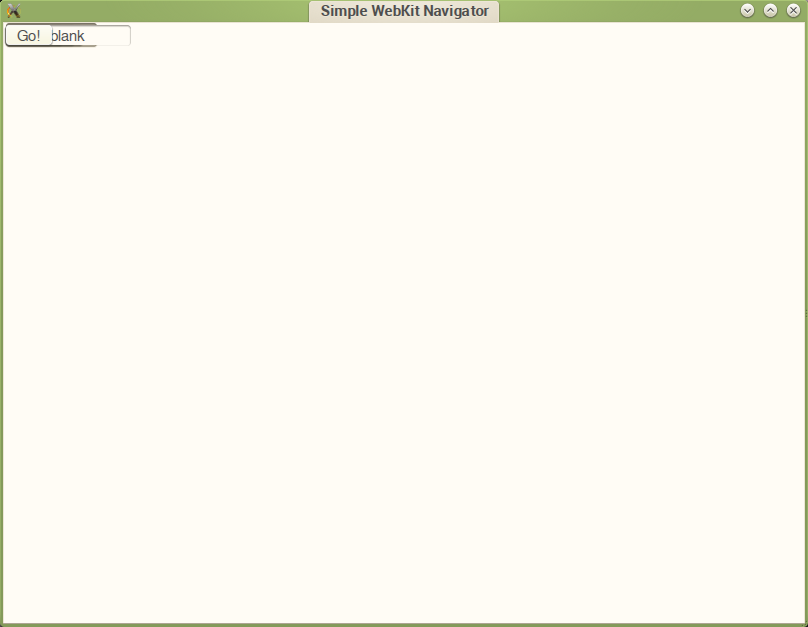
\includegraphics[scale=.5]{nolayout.png}
\caption{Application with no layout specified.}
\label{fig:nolayout}
\end{figure}
We are going to use two layouts in our web navigator widget: \li{QHBoxLayout} and \li{QVBoxLayout}.
There are also layouts for grids and forms.
In the \li{\_initUI()} method we need to append before \li{self.show()}
\begin{lstlisting}
navbar = QtGui.QHBoxLayout()
navbar.addWidget(back)
navbar.addWidget(forward)
navbar.addWidget(self.stop_reload)
navbar.addWidget(self.addr_bar)
navbar.addWidget(go_button)

vbox = QtGui.QVBoxLayout()
vbox.addLayout(navbar)
vbox.addWidget(self.wkctl)
vbox.addWidget(prob_bar)

self.setLayout(vbox)
\end{lstlisting}
Adding the layouts yields results in Figure \ref{fig:withlayout}.
\begin{figure}[h]
\centering
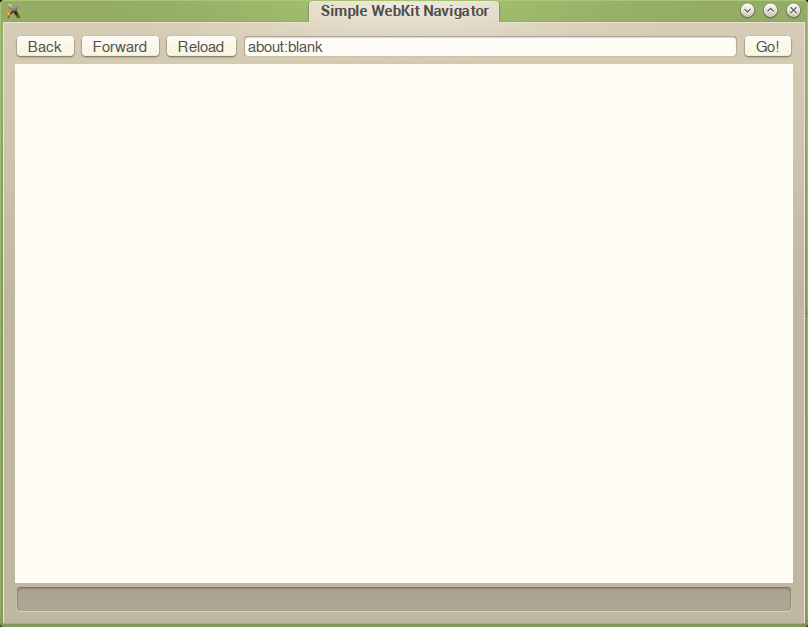
\includegraphics[scale=.5]{layout.png}
\caption{Application using a nested layout.
The controls in the navigation bar have their own layout which is nested into the first spot of the application-wide layout.}
\label{fig:withlayout}
\end{figure}

Structuring our program as a class allows us to very cleanly initialize a new application.
\begin{lstlisting}
def main():
    app = QtGui.QApplication(sys.argv)
    web = WebNavigator()
    sys.exit(app.exec_())
\end{lstlisting}
We first define a \li{QApplication} instance.
There can only a single \li{QApplication} object in existence at any time.
It initializes the context for all QWidget based applications.
It also manages the windows of the application and handles user input.
Next we instantiate our \li{WebNavigator} widget.
The last line starts the event handling loop and will exit Python when the application is terminated.
The completed program is listed below.
\lstinputlisting[style=fromfile]{webby.py}

\begin{problem}
Create a simple graphical user interface that will solve the quadratic formula given the necessary parameters.
Make the GUI look as below.
\begin{figure}[H]
\centering
\begin{subfigure}[b]{.49\textwidth}
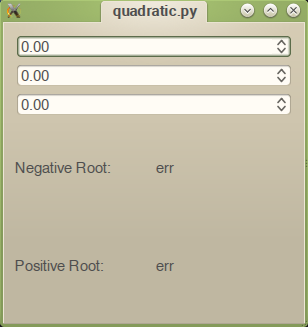
\includegraphics[width=\textwidth]{quadratic_view.png}
\end{subfigure}
\begin{subfigure}[b]{.49\textwidth}
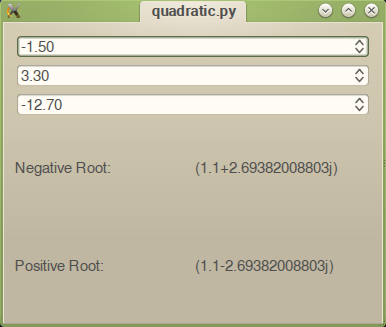
\includegraphics[width=\textwidth]{quadratic_view2.png}
\end{subfigure}
\end{figure}
The widgets that you will need are: \li{QDoubleSpinBox}, \li{QLabel}, \li{QGridLayout}, and \li{QVBoxLayout}.
You can view the documentation for these classes including all methods and signals at \url{http://qt-project.org/doc/qt-4.8/classes.html}
\end{problem}
